\paragraph{Histograma de gradientes orientados} ~\\
\label{subsection:hog}

	Los Histogramas de Gradientes Orientados o HOG (por sus siglas en inglés), son descriptores de características utilizados en visión por computadora y en el procesamiento de imágenes con el objetivo de realizar detección de objetos. Fueron introducidos por N. Dalal y B. Triggs en~\cite{DT05} con el propósito de realizar detección de personas; sin embargo, su uso no se limita solamente a esa área, sino que pueden ser utilizados en otras áreas como la detección de caracteres tal como hicieron Wang et al. en \cite{wang}.
	
	Todas las imágenes, como por ejemplo la presentada en la Figura~\ref{fig: Vector HOG}\textit{A}, contienen estructuras locales cuyas apariencias y formas pueden ser descritas por la distribución de los gradientes de intensidad como se puede observar en la Figura~\ref{fig: Vector HOG}\textit{B}.
	Un descriptor HOG es un vector compuesto por una combinación de histogramas que representan los gradientes de intensidad en distintas regiones de una imagen. La implementación de estos descriptores, se obtiene dividiendo a la imagen en regiones de tamaño fijo llamadas celdas, como se puede observar en la Figura~\ref{fig: Vector HOG}\textit{B}, y posteriormente, por cada celda, se calcula un histograma de gradientes para los píxeles en la celda ~\ref{fig: Vector HOG}\textit{C}.
	Luego, se agrupan las celdas en bloques (Figura \ref{fig: Vector HOG}\textit{C}) y se normaliza cada uno utilizando la norma \textit{L2}. Esto se hace con el objetivo de obtener un descriptor robusto ante los cambios en la iluminación entre otros. Consideremos la Figura \ref{fig: Vector HOG}\textit{C}, sea $b_{nm}~n,m=1,\dots,3$ un bloque $2 \times 2$ tal que 
	
	$$b_{nm} = (h_{nm}, h_{n(m+1)}, h_{(n+1)m}, h_{(n+1)(m+1)})$$
	
	En este ejemplo, $h_{ij}$ representa la celda ubicada en la fila $i$ columna $j$. Como se puede observar, en la figura aparece un área resaltada que hace referencia al bloque $b_{11}$. La norma \textit{L2} para $b_{11} = (h_{11}, h_{12}, h_{21}, h_{22})$ se obtiene de la siguiente manera:
	
	 $$||b_{11}||_2 = \sqrt{h_{11}^{2} + h_{12}^{2} + h_{21}^{2} + h_{22}^{2}}$$
	 luego se normaliza el bloque $b_{11}$ 
     $$b_{11}' = \frac{b_{11}}{||b_{11}||_2} $$
     
	 Finalmente, el descriptor HOG se obtiene de concatenar los histogramas obtenidos como muestra la Figura~\ref{fig: Vector HOG}\textit{D}.
	
	%El descriptor HOG mantiene una cuantas ventajas con respecto a otros métodos descriptores. Dado que el descriptor HOG opera en celdas localizadas, el método mantiene la invarianza a transformaciones geométricas y fotométricas, excepto para la orientación de objetos. Dichos cambios sólo aparecerían en regiones espaciales grandes~\cite{DT05}.
	
		\begin{figure}[htbp]
			\centering
			\centerline{ 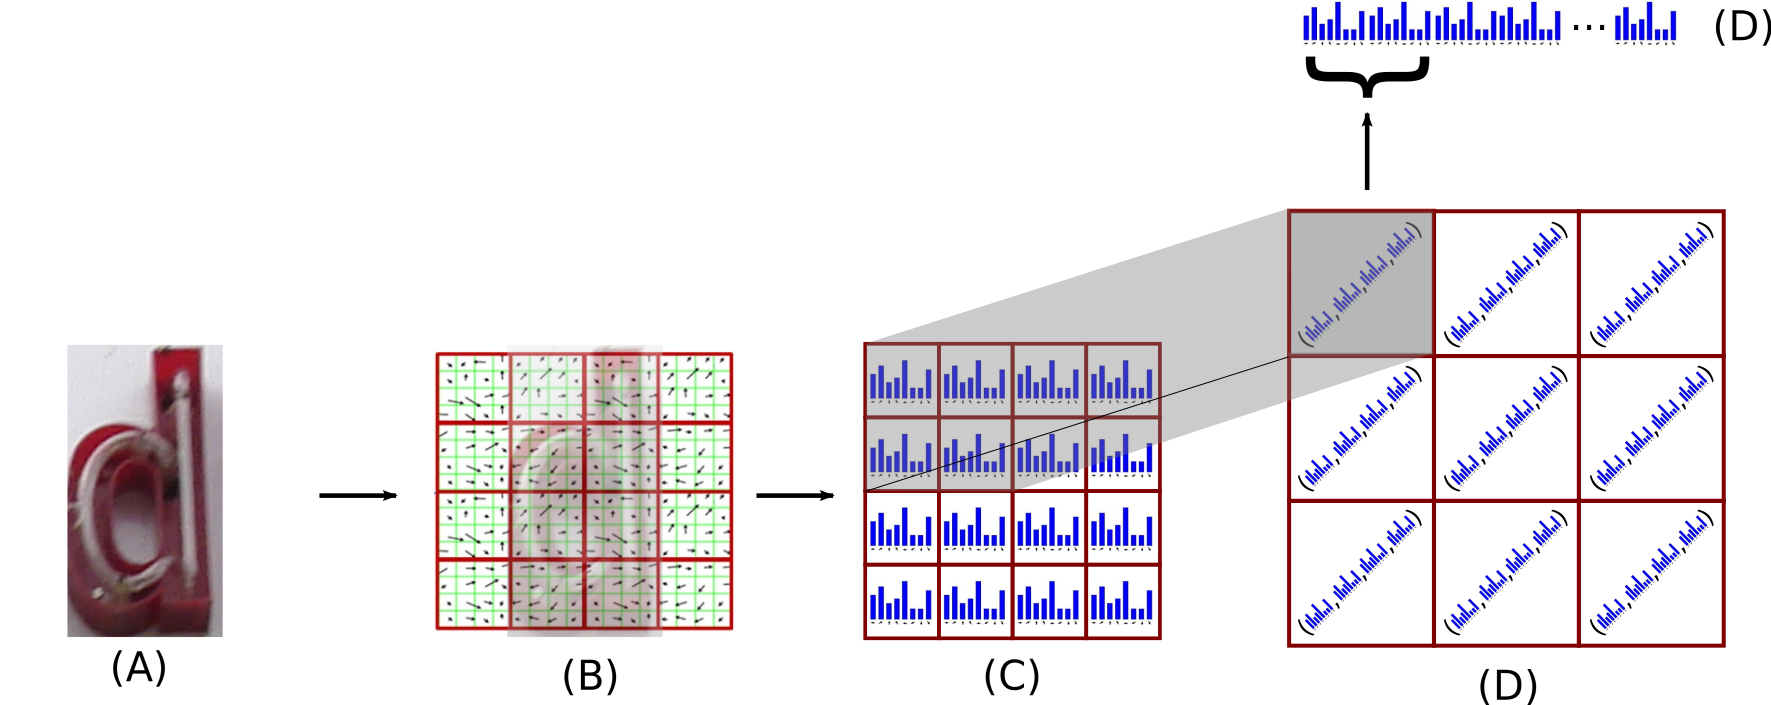
\includegraphics[scale=0.27]{img/hog/hog.png} }
			\caption[Extracción HOG]{Formación del vector de características HOG}
			\label{fig: Vector HOG}
		\end{figure}
		
	En el área de visión por computadora, los descriptores HOG son considerados estado del arte. Los mismos han demostrado ser útiles en la clasificación como se puede apreciar en el trabajo de Wang et al.~\cite{wang} donde se ha entrenado el clasificador Random Ferns con estos. Incluso, se puede decir que la performance obtenida con estos descriptores en dicho trabajo supera a la mayoría de los descriptores evaluados en el trabajo de De Campos et al.~\cite{dCBV09} bajo las mismas condiciones de entrenamiento.
	
	Una de las condiciones para poder usar los descriptores HOG en el clasificador \textit{Random Ferns}, es que los mismos tienen que estar binarizados. Los descriptores binarios son fáciles de computar, son compactos, se pueden almacenar fácilmente y son fáciles de comparar. En cambio, los descriptores originales tienen alta dimensionalidad y requieren sistemas con más memoria, capacidad de almacenamiento y procesamiento. Muchos sistemas en tiempo real como el reconocimiento de objetos~\cite{SJC08} y en el agrupamiento de puntos clave~\cite{OFL07} han incorporado este enfoque por su utilidad.

	
	\paragraph{Binarización} ~\\
	
		Como se dijo en \ref{subsection:ferns}, Random Ferns utiliza descriptores binarios tanto para el entrenamiento como para la evaluación del clasificador.
		
		Dado que los descriptores HOG no son binarios, es necesario establecer un método para su binarización. De esta forma es posible usarlos con Random Ferns. Para lograr esto se requiere de un vector umbral. El mismo, una vez  calculado, se encarga de binarizar todos los descriptores tanto del conjunto de entrenamiento como del conjunto de evaluación. Dicho umbral se calcula utilizando solamente el conjunto de entrenamiento y se obtiene de la siguiente manera:
		
		\begin{itemize}
		
			\item Dado $N$ descriptores HOG de dimensión $D$, se forma una matriz de tamaño $N \times D$ donde cada fila representa un vector.
			\item Se seleccionan $X$ columnas al azar de la matriz con reemplazo.
			\item Respetando el orden en que fueron seleccionadas, se aplica una función sobre cada columna (la función puede ser el calculo de la mediana, la media, bootstrap, entre otros). Se obtiene de esta manera un vector nuevo $W$ de dimensión $X$ tal que cada dimensión de $W$ está compuesta por un par $(z,y)$. $y$ es un número talque $0 \leq y \leq D$ que representa una de las columnas elegidas de la matriz y $z$ representa el valor resultante de haber aplicado la función elegida a dicha columna. Cabe aclarar que $X$ puede ser mayor o menor a $D$ por lo cual el umbral $W$ puede tener mayor o menor dimensión al final.
			\item Posteriormente dicho umbral $W$ se utiliza para binarizar los vectores originales de manera sencilla: sea $v_j$ con $j \in \{1,\dots,N\}$ uno de los $N$ vectores originales y tal que $v_j = d_1,d_2,\dots,d_D$. Luego se compara cada dimensión del umbral $W$ con la $y$-esima dimensión del vector $v_j$. Si $d_y \leq z$ se asigna 0, caso contrario 1. De esta manera binarizamos el vector $v_j$ obteniendo un nuevo vector binario de dimensión $X$.
			
		\end{itemize}

	Cada dimensión del vector umbral $W \in \mathbb{R}^{D}$ resulta de la aplicación de una función sobre una columna de la matriz de vectores. Dichas funciones representan los distintos métodos de binarización que se utilizan en el presente trabajo.
	
	A la binarización se la puede expresar con la siguiente composición de funciones:
	
	$$h \circ g:\mathbb{R}^{D} \rightarrow \{ 0, 1\}^{X}$$
	
	donde
	
	$$\textit{h: }\mathbb{R}^{X} \rightarrow \{ 0, 1\}^{X}$$
	
	$$\textit{g: }\mathbb{R}^{D} \rightarrow \mathbb{R}^{X}$$
	
	
	$\textit{g: }\mathbb{R}^{D} \rightarrow \mathbb{R}^{X}$ es una función definida de la siguiente manera. Dado un vector  $x=(x_1, \dots, x_D)$:

	\begin{equation}
	\label{eq: g_equation}
		g(x) = z = (z_1,\dots,z_X) \textit{ con } z_i=x_{\hat{i}},~\hat{i} \in \{1,\dots,D\}
	\end{equation}		
	
	En \ref{eq: g_equation} $\hat{i}$ representa un entero elegido de manera aleatoria en el rango $\{1,\dots,D\}$. Luego, un vez obtenido $z$, aplicamos la función $h$
	\begin{equation}
	\label{eq: h_equation}
		(y_1,\dots,y_X) = h(z) = (h_1(z_1),\dots,h_X(z_X))
	\end{equation}
	donde
	\[
    		h_{i}(z_i) = 
		\begin{cases}
    			1 & \text{si } z_i \geq u_{i}\\
    			0 & \text{caso contrario}
		\end{cases}
	\]

	$u_{i} \in \mathbb{R}$ representa al valor obtenido de haber aplicado una función de binarización a la columna \textit{i-esima} de la matriz  $N \times D$. Las funciones de binarización que se utilizan en este trabajo y que forman los vectores umbrales son: \textit{media}, \textit{mediana}, \textit{exponencial} y \textit{bootstrap}. A continuación se procede a explicar en detalle cada función.
	
	Dada la columna ``\textit{i-esima}'' de la matriz $N \times D$ representada por $C_i = (c_{i_1}, \dots, c_{i_j})$ con $j=1, \dots, N$ luego:

	\begin{itemize}
	
	\item \textbf{Media:}
	
	La \textbf{media} es una función de $\textit{b:}\mathbb{R}^{N} \rightarrow \mathbb{R}$ tal que:
	
	$$b(C_i) = \frac{\sum_{j=1}^N c_{i_j}}{N} $$

	\item \textbf{Mediana:}
	
	La \textbf{mediana} es una función de $\textit{b:}\mathbb{R}^{N} \rightarrow \mathbb{R}$ cuyo único requisito es que el vector esté ordenado. Sea \textit{dim(C)} la dimensión del vector $C$, luego:
	
	\[
    		b(C_i) = 
		\begin{cases}
    			\frac{c_{i_{\frac{dim(C)}{2}}} + c_{i_{\frac{dim(C)}{2}+1}}}{2} & \text{si dim(C) es par}\\
    			\frac{c_{i_{\frac{dim(C)}{2}}}}{2} & \text{caso contrario}
		\end{cases}
	\]
	
	\item \textbf{Bootstrap}
	
	Al igual que la \textit{media} y la \textit{mediana}, \textbf{bootstrap} es una función $\textit{b:}\mathbb{R}^{N} \rightarrow \mathbb{R}$ tal que, dado $c_{i_k} \in C_{i}$ una dimensión aleatoria de $C_{i}$ luego:
	
	$$ b(C_i) = c_{i_k} $$

	\item \textbf{Exponencial}
	
	La función \textbf{exponencial} $\textit{b:}\mathbb{R}^{N} \rightarrow \mathbb{R}$, surge de analizar la distribución de los datos para una columna de la matriz $N \times D$. Como se puede observar en la Figura Z, los datos del descriptor HOG extraidos de una imagen utilizada en el trabajo se justan a una distribución exponencial. Luego:
	
	\end{itemize}

	